\chapter{Results and Discussion}
The results and analysis is presented in this chapter. Section \ref{sec:performance_evaluation} presents the performance evaluation of COGMEN on MELD, IEMOCAP, and CMU-MOSEI, whereas results on personality prediction are described in Section \ref{sec:results_personality}. Section \ref{sec:emotion_distribution_analysis} and onwards entail the discussion and analysis of emotion distribution and personality prediction. Lastly, Section \ref{sec:current_limitations} presents current limitation with the work conducted in this study. 

\section{Results from Performance evaluation}
\label{sec:performance_evaluation}
Table \ref{tab:MELD-results} showcases the results of COGMEN on the MELD dataset \cite{HP_Advanced}. The model is run on a multimodal setting. The result show that COGMEN has best emotion prediction on the Neutral label and poorest on Disgust with F1 scores of 80.1\% and 12.9\%, respectively. Further, anger, disgust, and fear performs poorly. The reason to this problem is twofold: First, these three emotions have subtle differences resulting in misclassification of labels. Second, the MELD dataset suffers from class imbalance as stated in the original paper \cite{meld_dataset}.   
%
\begin{table}[h]
    \caption{Results on the MELD dataset for 7-emotion class. Avg. denotes the weighted average.}
    \centering
    \resizebox{\textwidth}{!}{%
    \begin{tabular}{|l|l|l|l|l|l|l|l|l|l|}
    \hline
        \multirow{}{}{Model} & \multicolumn{9}{c|}{\textbf{MELD}}  \\ \cline{2-10}
         &  Anger & Disgust & Sad & Joy & Neutral & Surprise & Fear & \multicolumn{2}{c|}{Avg.} \\ \cline{2-10} 
         & F1(\%) & F1(\%) & F1(\%) & F1(\%) & F1(\%) & F1(\%)& F1(\%) & F1(\%) & Acc.(\%)  \\ \hline \hline
         COGMEN & 49.5 & 12.9 & 51.2 & 65.2 & \textbf{80.1} & 72.0 & 21.0 & 65.2 & 65.55 \\ \hline
    \end{tabular}
    }
    \label{tab:MELD-results}
\end{table}
%
Experiments were performed on the IEMOCAP dataset for six emotion classes on multimodal setting \cite{HP_Advanced}. The results are showed in Table \ref{tab:IEMOCAP-results}. IEMOCAP achieves best weighted F1 score on the Sad emotion (80.4 \%). In addition, the poorest performance emotion is Happy (53.2\%).
%
\begin{table}[h]
    \caption{Results on the IEMOCAP dataset (6-way). Avg. denotes the weighted average.}
    \centering
    \resizebox{\textwidth}{!}{
    \begin{tabular}{|l|l|l|l|l|l|l|l|l|l|}
    \hline
        \multirow{}{}{Model} & \multicolumn{8}{c|}{\textbf{IEMOCAP}}  \\ \cline{2-9}
         &  Happy & Sad & Neutral & Angry & Excited & Frustrated & \multicolumn{2}{c|}{Avg.} \\ \cline{2-9} 
         & F1(\%) & F1(\%) & F1(\%) & F1(\%) & F1(\%) & F1(\%) & F1(\%) & Acc.(\%)  \\ \hline \hline
         COGMEN & 53.2 & \textbf{80.4} & 66.0 & 64.7  & 73.3 & 57.9 & 67.4 & 67.8 \\ \hline
    \end{tabular}
    }
    \label{tab:IEMOCAP-results}
\end{table}
%
For CMU-MOSEI, emotion classification across six emotion classes is performed using the Binary Classification setting \cite{COGMEN_joshi-etal-2022-cogmen}. The results on CMU-MOSEI are presented in Table \ref{tab:CMU-MOSEI-results}. COGMEN performs well on every emotion label where the best weighted F1 score is for the Fear label (88.1\%). The poorest score is for the Happy label, with a F1 of 70.2 \%. 
%
\begin{table}[h]
    \caption{Results on the CMU-MOSEI dataset (6-emotion class). Avg. denotes the weighted average.}
    \centering
    \resizebox{\textwidth}{!}{%
    \begin{tabular}{|l|l|l|l|l|l|l|l|l|l|}
    \hline
        \multirow{}{}{Model} & \multicolumn{8}{c|}{\textbf{CMU-MOSEI}}  \\ \cline{2-9}
         &  Happy & Sad & Angry & Fear & Disgust & Surprise & \multicolumn{2}{c|}{Avg.} \\ \cline{2-9} 
         & F1(\%) & F1(\%) & F1(\%) & F1(\%) & F1(\%) & F1(\%) & F1(\%) & Acc.(\%)  \\ \hline \hline
         COGMEN & 70.2 & 71.5 & 75.9 & \textbf{88.1}  & 82.6 & 83.4 & 75.9 & 76.2 \\ \hline
    \end{tabular}
    }
    \label{tab:CMU-MOSEI-results}
\end{table}
%
\\
The weighted average F1 and Accuracy scores of MELD, IEMOCAP, and CMU-MOSEI are compared in Table \ref{tab:datasets_results}. CMU-MOSEI outperforms IEMOCAP and MELD on F1 and accuracy by a great margin \cite{HP_Advanced}. However, the difference between IEMOCAP and MELD is only 2.2\% and 2.25\%. This suggests that COGMEN is generalizable across different datasets. 
%
\begin{table}[h]
\caption{Comparison of COGMEN performed on the three datasets.}
\centering
\resizebox{2.3in}{!}{%
\begin{tabular}{|l|l|l|}
\hline
\multicolumn{1}{|c|}{\textbf{Name}} & \multicolumn{1}{c|}{\textbf{F1}} & \multicolumn{1}{c|}{\textbf{Accuracy}} \\ \hline
MELD & 65.2 & 65.55\\ \hline
IEMOCAP & 67.4 & 67.8 \\ \hline
CMU-MOSEI & 75.9 & 76.2 \\ \hline
\end{tabular}
}
\label{tab:datasets_results}
\end{table}
%
\\
With the presented results in this section, it seems natural to select CMU-MOSEI for training the AVI dataset given the performance. However, there are several reasons why the AVI dataset is trained on IEMOCAP in a mulimodal setting. First, following the work presented in \cite{cmu-mosei_zadeh2018multimodal}, it was impossible to extract visual features as FaceNet 2.0 is not open-source. Therefore, the feature extraction pipeline was created obeying IEMOCAP procedure. Second, the most important reason was that CMU-MOSEI does not have neutral label for the 6-emotion class. As the neutral emotion is essential for predicting the likelihood of certain personality traits, IEMOCAP was used. 


\section{Results on personality prediction}
\label{sec:results_personality}
COGMEN, which is the state-of-the-art model for emotion recognition, was used to retrieve emotion expressed in the interviews. The model was trained on the IEMOCAP benchmark, as it is most appropriate for this thesis study. \\

Figure \ref{fig:emotion_personality_all} shows side-by-side the emotion distribution and predicted personality traits for each participant. The emotions are normalized in to 0 -- 1 by the sum of an emotion per video over the total number of emotions for a given video. The predicted behavioral traits are presented in descending order, where the strongest trait is introduced first. As can be seen from the graphs illustrated in Figure \ref{fig:emotion_personality_all}, candidates show a happy emotion in a small portion of the interview. There were also interviews where no happy emotion was elicited, as for sample 2, sample 4, sample 6, and sample 7, respectively. It is interesting to note that negative or neutral feeling are the most dominant across all samples except from sample 5, who has equal distribution of excited and sad. For personality prediction, the most reoccurring traits predicted are conscientiousness, openness, and neuroticism, respectively. Extraversion is only forecasted in one sample. 
\newpage
\begin{figure}[h!]
  \centering
  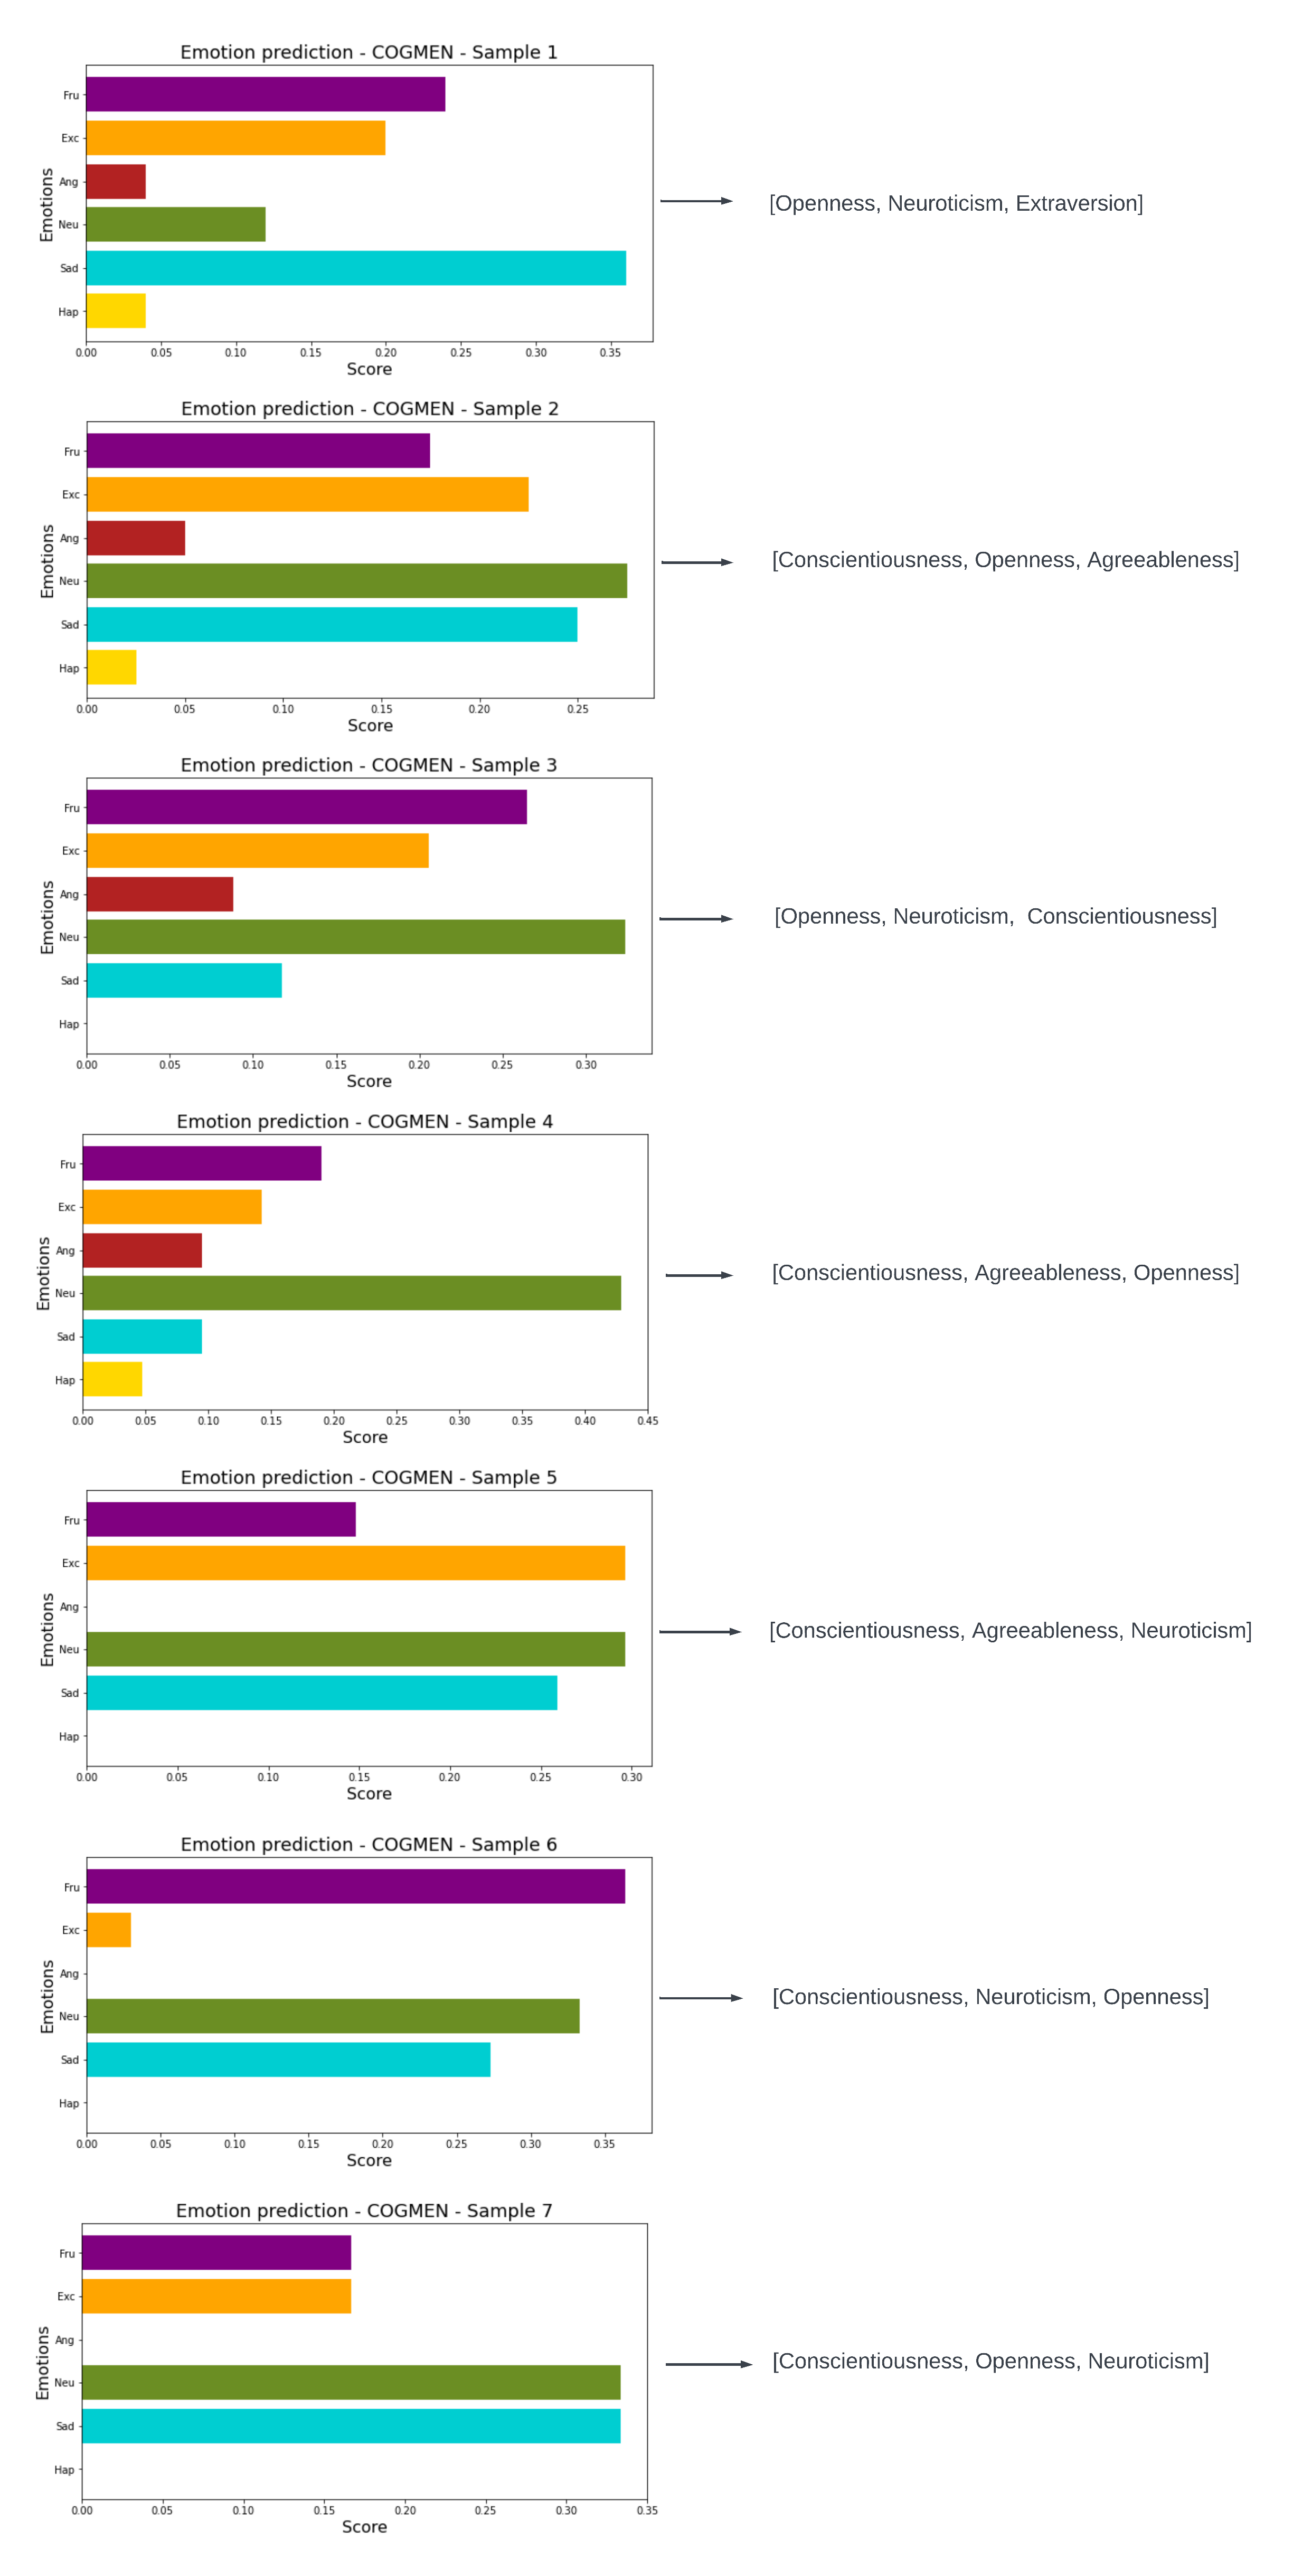
\includegraphics[width=\linewidth, height=0.9\textheight]{figures/emotion_personality_7.png}
  \caption{Emotion distribution and predicted personality traits.}
  \label{fig:emotion_personality_all}
\end{figure}

\section{Emotion distribution analysis across samples}
\label{sec:emotion_distribution_analysis}
Figure \ref{fig:emotion_distribution} gives an overview of the emotion distribution of participant P1-P7. The emotions are normalized to 0 -- 1. As can be seen from Figure \ref{fig:emotion_distribution}, participants tend to be more excited than happy during the interview. For negative emotions, sad and frustrated are most dominant across samples, whereas angry is expressed to a lesser extent. The neutral emotion is elicited the most in candidates except sample 1. 
%
\begin{figure}[h]
  \centering
  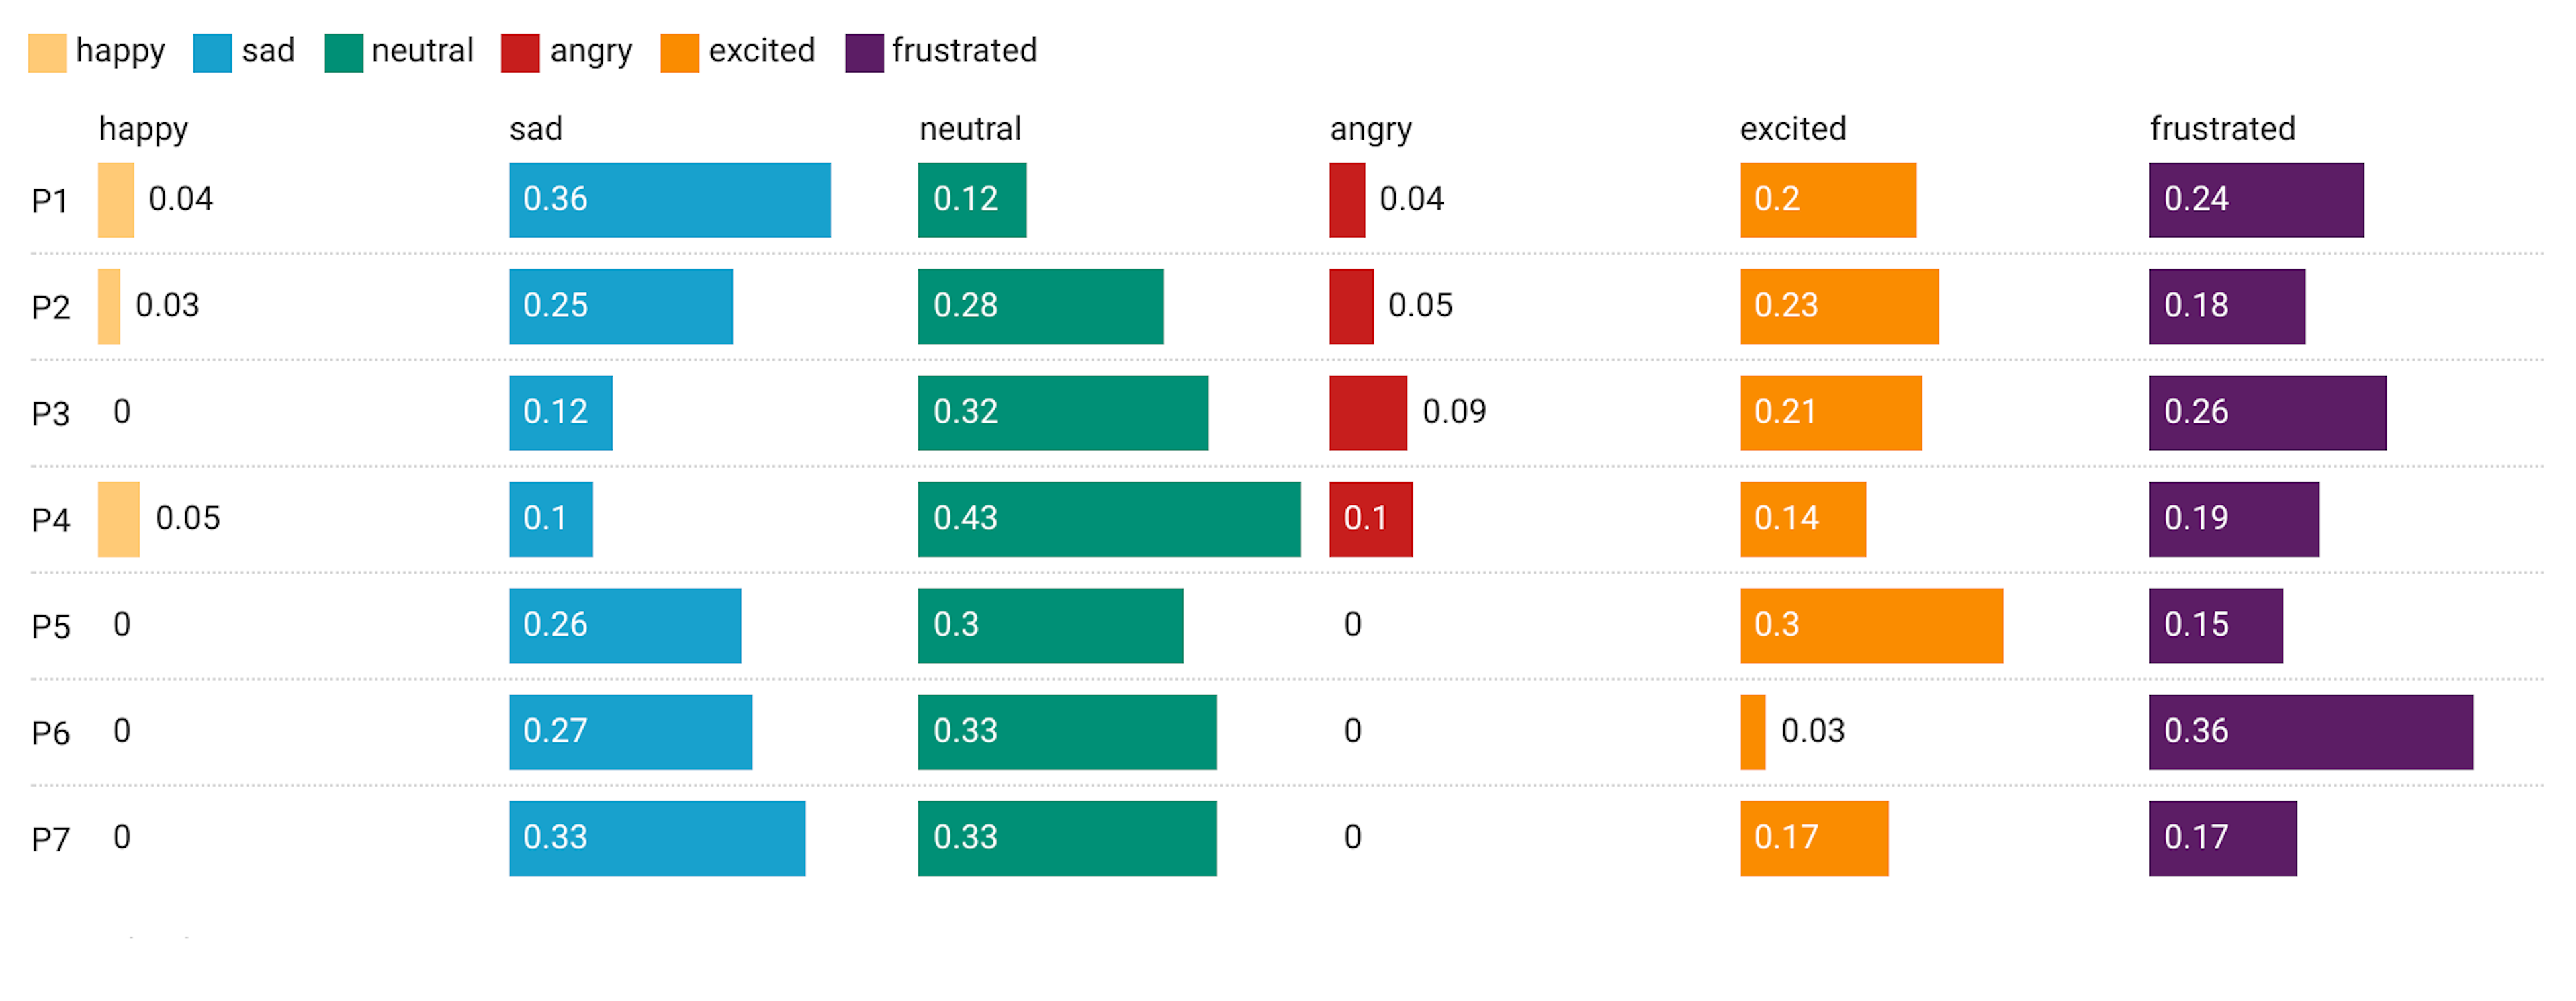
\includegraphics[width=\textwidth]{figures/emotion_dist_all.png}
  \caption{Emotion distribution for participants.}
  \label{fig:emotion_distribution}
\end{figure}
%
The reason for this emotion distribution is reflected in the AVI design features. First of all, this interview setting may be new to the participants and they do not know what to expect from it. Therefore, it is natural to assume candidates are dealing with interview nerves to some extent. Another factor that may increase uncertainty among applicants is interview questions not being shown to them until right before the recording happens. As a result, the participants are unable to unveil to much emotions. During the interview, candidates are allowed to re-record each response up to three times and select the answer they find most significant. Although this feature mitigates interview nerves and increases fairness perception, it does not mean applicants are expressing more emotions in sophisticated responses. The interview questions are the most important feature for the emotion distribution. In general, the questions are challenging and require the participants to reflect and discuss earlier endeavours. The four inquiries are separated into two questions entailing positive experience and two questions about facing a challenge or problem. For that reason, all six emotions are more or less represented in the AVIs. 

\section{Personality prediction analysis}
Figure \ref{fig:personality_distribution} depicts the scores for participant (P1-P7). The personalty score ranges from 0 -- 1.2. By comparing the predicted results with the test scores, the personality prediction models achieves 44 \% accuracy in predicting the three strongest traits in right order, and the approach achieves 67 \% accuracy predicting the strongest traits regardless of the order. In sample 4, the three strongest traits are predicted the same a the Big Five test. However, in sample 3, only one label is predicted right. It is interesting to see the high covariance between conscientiousness and agreeableness. These results support the previous conducted studies that these two traits move in line with each others as they have overlapping characteristics. Based on the findings, it is challenging to predict agreeableness solely on happiness and excited, and thus is this correlation an important factor when analyzing the emotion distribution. 
%
\begin{figure}[h]
  \centering
  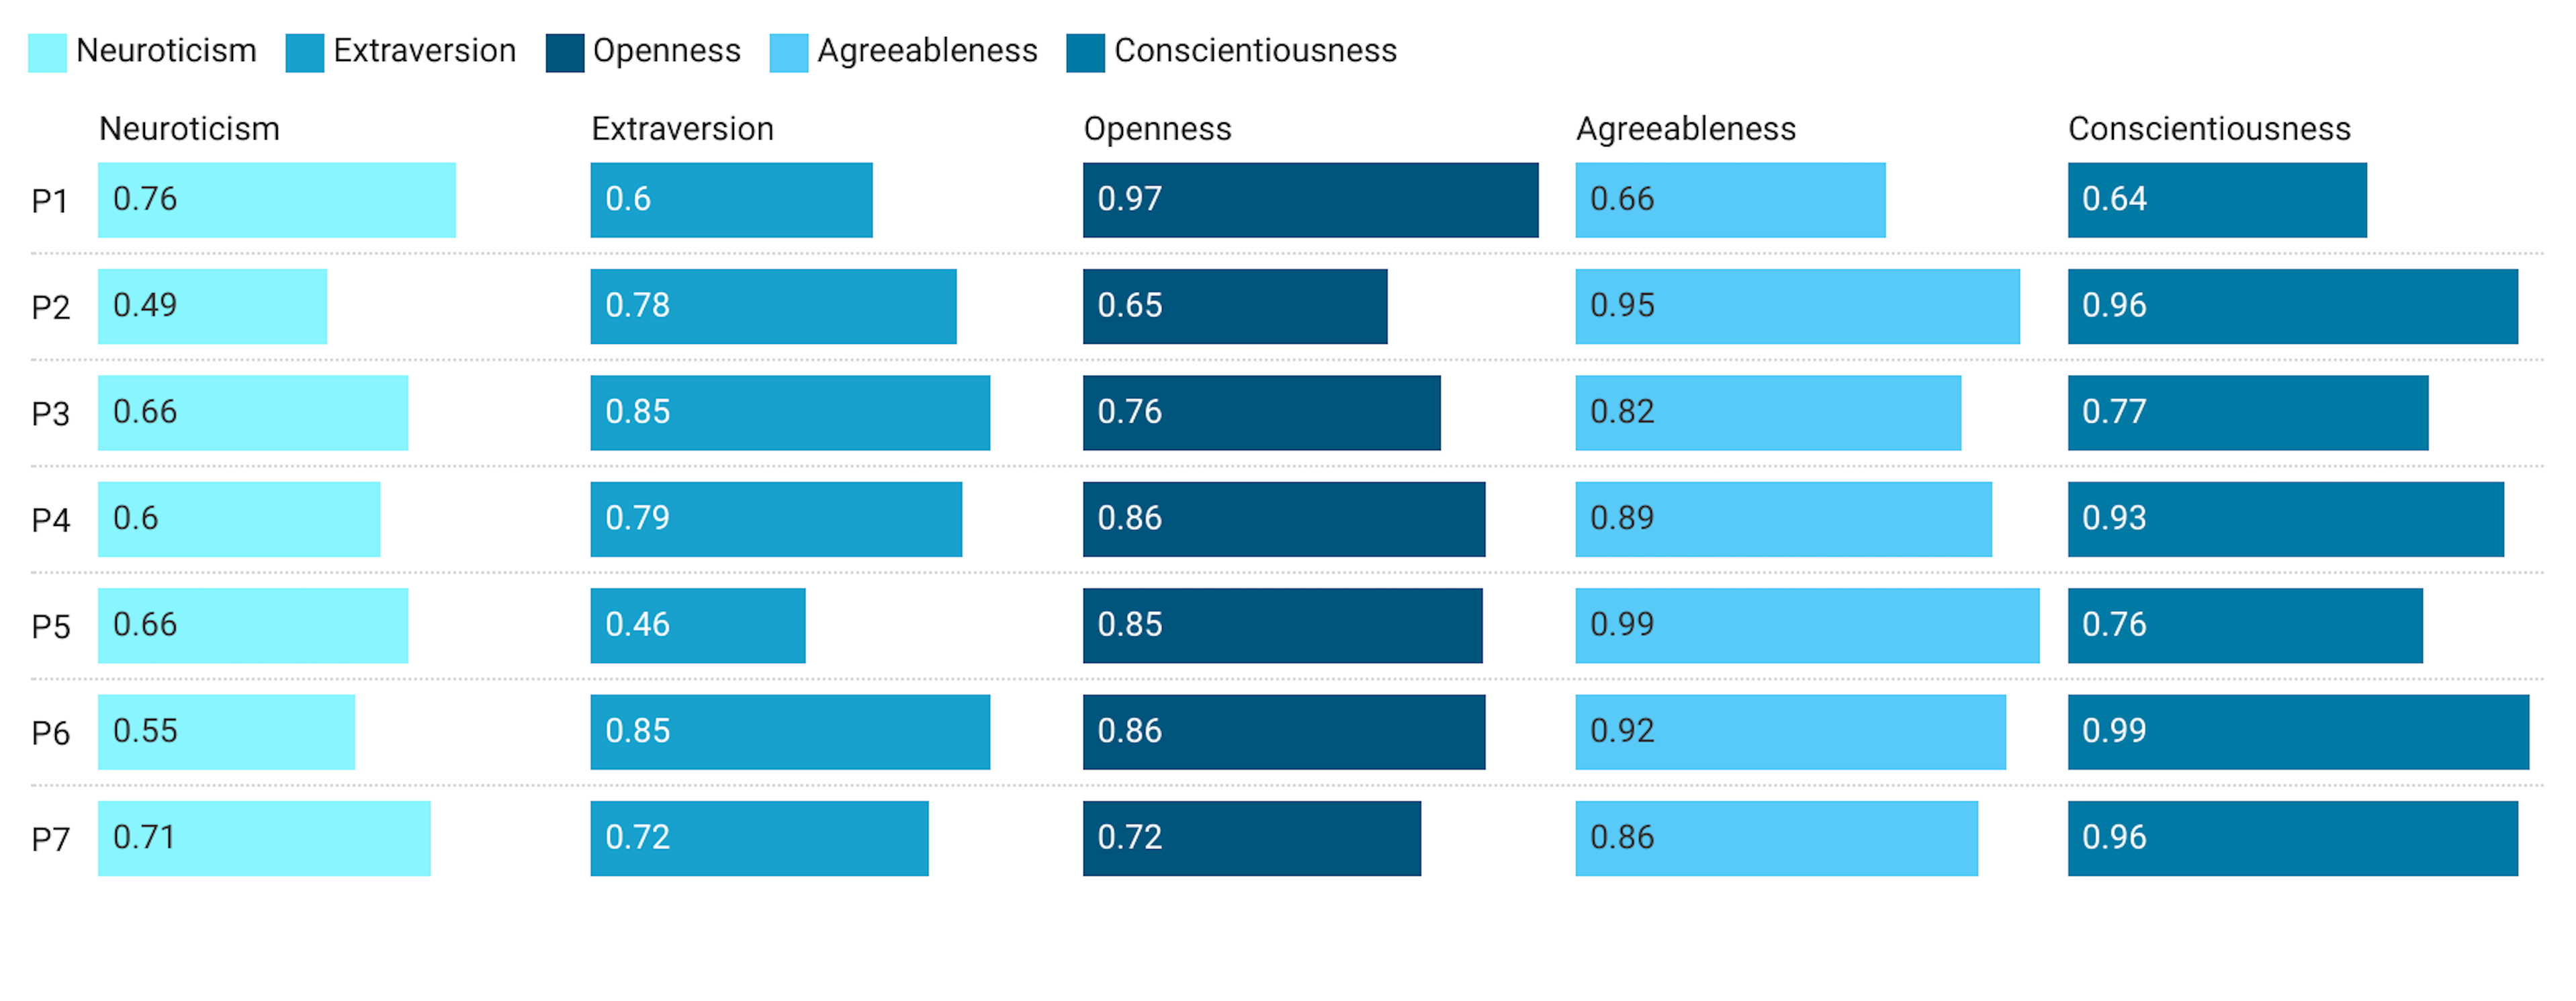
\includegraphics[width=\textwidth]{figures/personality_dist_all.png}
  \caption{Personality distribution based on Big Five personality test.}
  \label{fig:personality_distribution}
\end{figure}
%
In the case of neuroticism, one participant has the trait as one of the three strongest. Still, the personality likelihood model predicts neuroticism in four of the six samples. The reason is that there is a high degree of negative emotions of these participants during the interview. Extraversion is the least predicted trait from the approach. Nevertheless, applicants including P3, P4, and P6 have high scores in extraversion. The interview setting fails to capture if someone is extrovert/introvert because candidates response the interview questions without any back-and-forth communication stream. Although extraversion is associated with a higher positive effect, the personality prediction is not able to distinguish extraversion from agreeableness. Therefore, it is neccesary to facilitate the recruitment process with other activities in order to get a full grasp of each applicant. Assessing extraversion in candidates can be performed during group interviews or assessment centers where physical attendance is required. 

\subsection{Emotion transition analysis for interview questions}
It was observed in Figure \ref{fig:emotion_distribution} that the emotion distribution differs in the participants. The emotion distribution is further analyzed by looking at the emotion grouping for each question. Emotion transitions per question for each participant is presented in Figure \ref{fig:emotion_transition_questions}. The graph shows what emotions are expressed at a particular question. The colors represent the emotion transition, y-axis shows each emotion, and the x-axis depicts the clips from start to end. It is important to note that number of clips are different for the participants, since the interview duration is different for the applicants. To recall, the interview questions used in the AVI dataset are:
%
\begin{figure}[h]
  \centering
  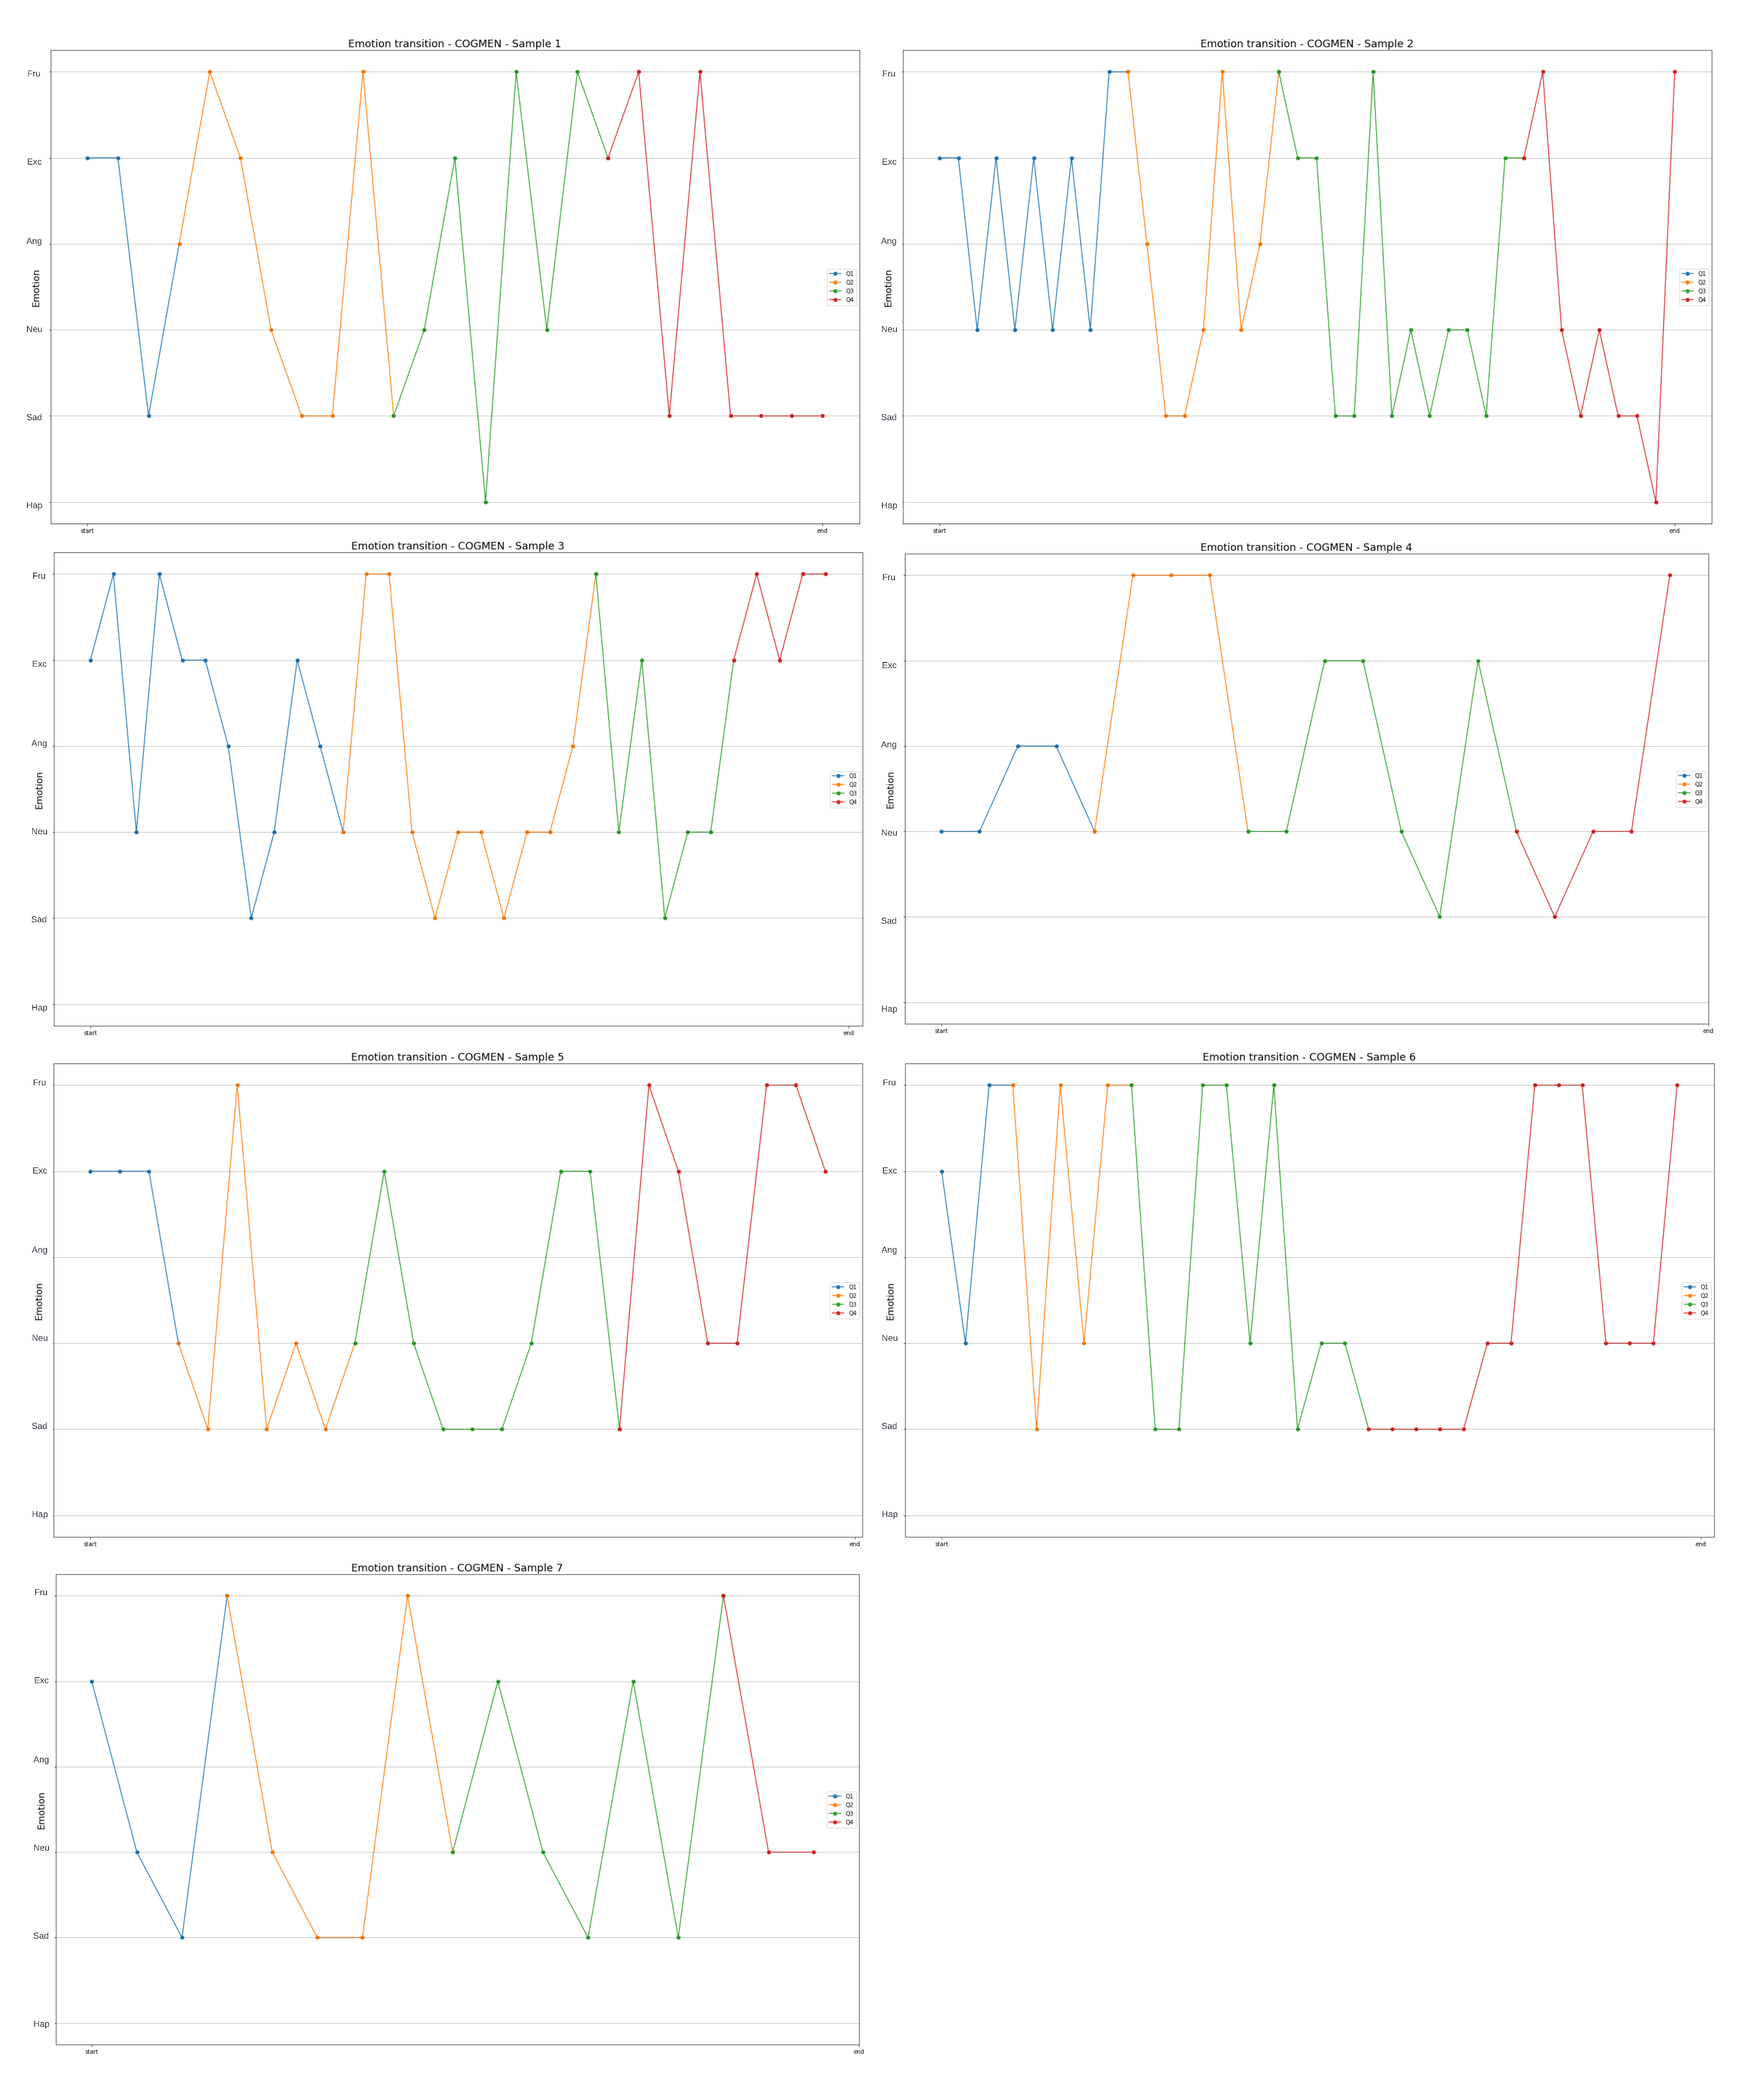
\includegraphics[width=\textwidth]{figures/emotion_transition_questions.png}
  \caption{Emotion distribution for each interview question.}
  \label{fig:emotion_transition_questions}
\end{figure}
%
%
\begin{itemize}
    \item[] Q1: What motivates you? What are you passionate about?
    \item[] Q2: Not everyone agrees all the time. Have you had a peer, teammate or friend disagree with you? What did you do?
    \item[] Q3: Give an example of a time you have gone over and above to achieve something. Why was it important for you to achieve this?
    \item[] Q4: Sometimes things don’t always go to plan. Describe a time when you failed to meet a deadline or personal commitment. What did you do? How did that make you feel? 
\end{itemize}
%
As stated in Section \ref{sec:video_interview}, these questions are based on past behavior, situational judgement, and their nature will oblige candidates to express various emotions. As can bee seen from Figure \ref{fig:emotion_transition_questions}, for Q1, excited and neutral are the most dominating traits. Q2 and Q4 unveil most negative affect in applicants, where sad is most expressed. Although Q3 is associated with a positive experience, the trend is that candidates deliberate negative emotions (i.e. sad, and frustrated). The reason could be that applicants reflect on the process and share how they felt facing that problem. It is interesting to note that the candidates who score high in conscientiousness (e.g. P2, P4, and P6) exhibits much neutral emotion when discussing accomplishments (Q1 and Q3). This supports the research that people who are conscientious tend to discuss achievements more than people with low in conscientiousness \cite{conscientiousness1-HIRSH2009524}. In addition, this confirms that the neutral emotion can be used to predict the likelihood of a candidate's level of conscientiousness. 

\section{Correlation Analysis}
Given the lack of emotion labels for the AVI dataset, the predicted emotion distribution is dependent on COGMEN's performance. Consequently, COGMEN is compared with two baselines, bc-LSTM\cite{bc-LSTM_poria2017context} and DialogueRNN \cite{DialogueRNN_MAJUMDER2018124}. These models aim to solve the same challenge as COGMEN, but using different deep learning architectures. In particular, there are three reasons why the two model were chosen. First, both models are open-source and available via GitHub. Second, both bc-LSTM and DialogueRNN are trained and tested on IEMOCAP, achieving competitive performance with COGMEN. The final reason is that these frameworks facilitates to be incorporated with the established feature extraction procedure explained in Section \ref{sec:feature_extraction}. The Pearson correlation between MSA models is analyzed to see the emotion distribution similarities. 
%
\begin{table}[h]
\caption{Correlation for emotions distribution between MSA models.}
\centering
\resizebox{\columnwidth}{!}{%
\begin{tabular}{|l|l|l|l|l|l|l|l|l|l|}
\hline
\multicolumn{1}{|c|}{No.} & \multicolumn{1}{c|}{Correlation b/w} & \multicolumn{1}{c|}{Happy} & \multicolumn{1}{c|}{Sad} & \multicolumn{1}{c|}{Neutral}  & \multicolumn{1}{c|}{Angry} & \multicolumn{1}{c|}{Excited} & \multicolumn{1}{c|}{Frustrated}\\ \hline
 1 & COGMEN--bc-LSTM & 0.940 & 0.960 & 0.866 & 0.840 & 0.934 & 0.781 \\ \hline
 2 & COGMEN--DialogueRNN & 0.890 & 0.844 & 0.729 & 0.870 & 0.921 & 0.722 \\ \hline
\end{tabular}
}
\label{tab:correlation_analysis}
\end{table}
%
As can be seen from Table \ref{tab:correlation_analysis}, there is a high correlation between COGMEN and bc-LSTM as well as for COGMEN-DialogueRNN. However, COGMEN--DialogueRNN have a slightly poorer correlation than COGMEN--bc-LSTM. A possible reason for this is that DialogueRNN have lesser performance on IEMOCAP compared to bc-LSTM. When that is said, all three MSA models reflect the same emotion distribution from the AVIs. This means that predicted behavioral traits remain the same independently of MSA model. As a result, this analysis validates COGMEN's emotion prediction in the study. 

\section{Findings concerning RQ's}
Following the detected personality traits by the proposed model and the analysis of results presented in previous subsections, for (RQ1), it is safe to assume that MSA can assist in predicting personality traits from the Big Five taxonomy. By examining the emotion expressed by participants and comparing with the validation criteria, the model performs well in predicting the three strongest traits in candidates. It is still difficult to say to what extent, as this research is exploring one working domain as well as the number of participant is far less than for any statistically significant observations. (RQ2) The emotion distribution in an interview is the most essential parameter to analyze in order to predict human attributes. However, in the case of this study, sad, neutral, excited, and frustrated are the most relevant emotions for personality classification, whereas happy and angry were hardly expressed by the interviewees. (RQ3) In fact, it was observed that sentiments are useful in personality prediction. Since the findings conveyed that no emotions were directly linked to each distinct personality trait, the distribution of positive and negative sentiments is convenient when predicting human attributes. (RQ4) Especially agreeableness and extraversion are difficult to predict based on MSA in an AVI setting. The former has a relationship to positive emotions as well as a correlation to conscientiousness. The latter is also associated with positive effect and therefore challenging to distinguish from agreeableness. Additionally, the interview setting fails to capture the characteristics of extraversion, because the applicants are only leading a one-sided conversation. Extraversion, in particular, is easier to predict in other recruitment activities such as group interviews and during assessment centres. (RQ5) It was observed that people from the informatics domain score high in conscientiousness and agreeableness. The lowest trait in the candidates is neuroticism, whereas extraversion and openness seem to vary between applicants. 

\section{Current limitations}
\label{sec:current_limitations}
Although, the work carried out in this thesis draws a reasonable portrait of how MSA assist personality prediction in AVIs, however it is impossible to cover all aspects regarding MSA and contemporary psychology. The limitations of this study are as follows:
%
\begin{enumerate}
    \item This work collects a dataset, namely AVI dataset, to investigate how MSA can be used for personality prediction in AVIs. The dataset lacks ground truth i.e. labeled emotions for each utterance. Therefore, the emotion distribution is based on COGMEN's performance. To validate the emotion expressed in the interviews, two MSA baselines are utilized to compare their emotion distributions. 
    \item The AVI dataset lacks ground truth data i.e. personality likelihood of each utterance. For that reason, the proposed personality prediction approach is based on emotions-personality relationship research. The personality prediction method is validated by the use of Big Five personality questionnaire. 
    \item The AVI dataset has seven speakers from the informatics domain resulting in a total length of approximately 40 minutes. The sample size is to low in order to becoming a benchmark. However, since this qualitative research investigates the personality of informatics students, the sample size is sufficient to describe the phenomenon of interest and answer the RQ's at hand. 
    \item The demographics of the participants is limited to Norway, meaning that the applicants use English as a second language. This can affect the predicted emotion distribution as people whose mother tongue is English have an apparently wider vocabulary. In addition, it would be interesting to compare the emotions expressed from different countries, as research supports that people across the world reason differently. 
    \item The response preparation time AVI setting is an element of uncertainty for the data acquisition. As stated in the experiment instructions (Section \ref{sec:video_interview}), candidate can view the interview questions right before the recording happens. However, there exists no mechanism to ensure this principle is held. The facilitators trust that candidates follow the provided instructions. If the participants choose to practise the responses, the only disadvantage is that they will communicate more sophisticated interview answers. 
\end{enumerate}
%

\begin{comment}
\begin{table}[h]
    \caption{Results on the IEMOCAP dataset (6-way).}
    \centering
    \resizebox{\textwidth}{!}{%
    \begin{tabular}{|l|l|l|l|l|l|l|l|l|l|}
    \hline
        \multirow{}{}{Model} & \multicolumn{8}{c|}{\textbf{IEMOCAP}}  \\ \cline{2-9}
         &  Happy & Sad & Neutral & Angry & Excited & Frustrated & \multicolumn{2}{c|}{Avg.} \\ \cline{2-9} 
         & F1(\%) & F1(\%) & F1(\%) & F1(\%) & F1(\%) & F1(\%) & F1(\%) & Acc.(\%)  \\ \hline \hline
         COGMEN & 53.2 & \textbf{80.4} & 66.0 & 64.7  & 73.3 & 57.9 & 67.4 & 67.8 \\ \hline
    \end{tabular}
    }
    \label{tab:IEMOCAP-results}
\end{table}
%
\begin{table}[h]
    \caption{Results on the MELD dataset for 7-emotion class. Avg. denotes the weighted average.}
    \centering
    \resizebox{\textwidth}{!}{%
    \begin{tabular}{|l|l|l|l|l|l|l|l|l|l|}
    \hline
        \multirow{}{}{Model} & \multicolumn{9}{c|}{\textbf{MELD}}  \\ \cline{2-10}
         &  Anger & Disgust & Sad & Joy & Neutral & Surprise & Fear & \multicolumn{2}{c|}{Avg.} \\ \cline{2-10} 
         & F1(\%) & F1(\%) & F1(\%) & F1(\%) & F1(\%) & F1(\%)& F1(\%) & F1(\%) & Acc.(\%)  \\ \hline \hline
         COGMEN & 49.5 & 12.9 & 51.2 & 65.2 & \textbf{80.1} & 72.0 & 21.0 & 65.2 & 65.55 \\ \hline
    \end{tabular}
    }
    \label{tab:MELD-results}
\end{table}
%
%
\begin{table}[h]
    \caption{Results on the CMU-MOSEI dataset (6-emotion class).} Avg. denotes the weighted average.
    \centering
    \resizebox{\textwidth}{!}{%
    \begin{tabular}{|l|l|l|l|l|l|l|l|l|l|}
    \hline
        \multirow{}{}{Model} & \multicolumn{8}{c|}{\textbf{CMU-MOSEI}}  \\ \cline{2-9}
         &  Happy & Sad & Angry & Fear & Disgust & Surprise & \multicolumn{2}{c|}{Avg.} \\ \cline{2-9} 
         & F1(\%) & F1(\%) & F1(\%) & F1(\%) & F1(\%) & F1(\%) & F1(\%) & Acc.(\%)  \\ \hline \hline
         COGMEN & 70.2 & 71.5 & 75.9 & \textbf{88.1}  & 82.6 & 83.4 & 75.9 & 76.2 \\ \hline
    \end{tabular}
    }
    \label{tab:CMU-MOSEI-results}
\end{table}
%
\end{comment}
       